\documentclass[tikz,border=10pt]{standalone}%
\usetikzlibrary{arrows.meta,bending,positioning}%
\begin{document}%
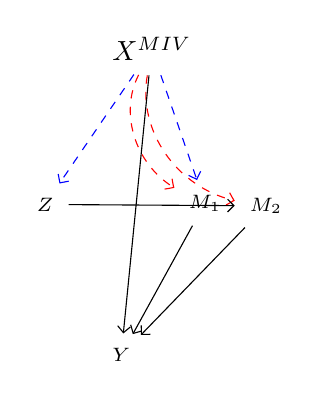
\begin{tikzpicture}[%
  node distance=1.5cm and 0.5cm,%
  every node/.style={font=\scriptsize},%
  arrow/.style={-{Straight Barb[bend]},shorten >=2pt,shorten <=2pt},%
  MIV/.style={name=MIV,font=\bfseries},%
  every edge/.append style={arrow}%
]%
  \node [MIV] (MIV) {$X^{MIV}$};%
  \node [below left=of MIV] (Z) {$Z$};%
  \node [below right=of MIV] (M2) {$M_2$};%
  \node [below right=of Z] (Y) {$Y$};%
  \node [above right=of Y] (M1) {$M_1$};%
  \draw [dashed,blue] (MIV) edge (Z) (MIV) edge (M1);%
  \draw [dashed,red,bend right=45] (MIV) edge (M2) (MIV) edge (M1);%
  \draw (Z) edge (M2) (M1) edge (Y) (M2) edge (Y) (MIV) edge (Y);%
\end{tikzpicture}%
\end{document}